\documentclass[11pt,twoside,twocolumn,a4paper]{article}

\usepackage{acvrw}
\usepackage{times}
\usepackage{epsfig}
\usepackage{graphicx}
\usepackage{amsmath}
\usepackage{amssymb}
\usepackage{url}
\usepackage{float}

\newcommand\scalemath[2]{\scalebox{#1}{\mbox{\ensuremath{\displaystyle #2}}}}

%%%%%%%%%%%%%%%
%% FINAL COPY %
%%%%%%%%%%%%%%%

% !!! UNCOMMENT THIS LINE FOR THE FINAL SUBMISSION !!!
% \acvrwfinalcopy 

\def\acvrwPaperID{20} % *** Enter the ACVRW Paper ID here
\def\httilde{\mbox{\tt\raisebox{-.5ex}{\symbol{126}}}}

% Pages are numbered in submission mode, and unnumbered in camera-ready
\ifacvrwfinal\pagestyle{empty}\fi
\begin{document}


%%%%%%%%%
% TITLE %
%%%%%%%%%
\title{Object Tracking Robot using Stereo Vision}


\author{Nicolai Schwartze, Johannes Wüstner\\
FH Vorarlberg University of Applied Science\\
{\tt\small \{nicolai.schwartze,johannes.wuestner\}@students.fhv.at}
}


\maketitle
\ifacvrwfinal\thispagestyle{fancy}\fi

%%%%%%%%%%%%
% ABSTRACT %
%%%%%%%%%%%%

\begin{abstract}
This paper originates from a coursework done in the module Applied Robotics at the Vorarlberg University of Applied Science (FH Vorarlberg). The work is about finding a green laser point on a white flip-board chart. A robot with a 3D camera system tracks this point and drives its laser-pointer tool to the same spot. The premiss was not to use any position controller and instead compute the desired axis-angles from the 3D information of the found laser dot. The paper describes the design and the implementation of the system. 
\end{abstract}


%%%%%%%%%%%%%
% BODY TEXT %
%%%%%%%%%%%%%

%-------------------------------------------------------------------------
\section{Task Constrains}

The following requirements were posed to fulfil this coursework: 
\begin{itemize}
\item Create a 3-axis robot and not a simple two-axis pan/tilt device. 
\item Measure the 3D point of the laser and drive to its position without using a closed loop controller. 
\end{itemize}

%-------------------------------------------------------------------------
\section{Design}

The robot consists of 3 Dynamixel MX-64AT motors, two Microsoft Lifecam HD 3000 (640x480 pixel) and a laser-pointer.
Aluminium frames are attached to the motors to build the framework of the robot. The cameras and laser-pointer are connected with aluminium brackets. The design of the robot and its components is established with SolidWorks.
Figure \ref{fig:3d-render} shows a 3D render of the fully assembled robot.

\begin{figure}[h]
	\centering
	\includegraphics[width=0.3\columnwidth]{images/robot_3D_side.pdf}
	\caption{3D render of the assembled robot}
	\label{fig:3d-render}
\end{figure}



%-----------------------------------------------------------------------------
\section{Robot Kinematic}

The motors can be controlled by a supplied library, which is written in C \cite{Robotis2019}. This allows us to write our own DLL to implement the backwards kinematics and control the robot as a whole. Figure \ref{fig:robot-axis-coord} shows the coordinate systems that are used to get the link parameters shown in table \ref{tab:link_parameter}. The link parameters are established using the Denavit Hartenberg convention mentioned in \cite[p. 70-79]{Craig2018}.


With the link parameters, the inverse kinematics matrix can be generated. This is used to transfer the 3D point captured by the camera, from the tool frame $\left\lbrace F \right\rbrace$  to the base coordinate system $\left\lbrace 0 \right\rbrace $. From there, the point can be transferred into the coordinate frame $\left\lbrace 3 \right\rbrace $. This transformation is implicitly included in equation (\ref{eq:theta2}). Together with (\ref{eq:theta0}) these equations can be used to calculate the desired robot configuration. 
Because $\theta_1$ and $\theta_2$ directly depend on each other, $\theta_1$ can be set to any arbitrary angle.

\begin{equation}
\label{eq:theta0}
\theta_0 = arctan \left(  \frac{P_{Y0}}{P_{X0}} \right) 
\end{equation}

\begin{equation}
\label{eq:theta2}
\theta_2 = - arctan \left( \frac{ P_{Z0} - 100 - 100 cos(\theta_1)}{\sqrt{P_{X0}^{2} + P_{Y0}^{2}} - 50 - 100 sin(\theta_1)} \right)
\end{equation}

\begin{table}[h]
	\centering
	\begin{tabular}{ | c | c | c | c | c | }
		\hline
		$i$ & $\alpha_{i-1}$ & $a_{i-1}$ & $d_i$ & $\theta_{i-1}$\\ 
		\hline \hline
		1 & 0 & 0 & 100 & $\theta_0$\\  
		2 & -90 & 50 & 0 & $\theta_1 - 90$\\ 
		3 & 0 & 100 & 0 & $\theta_2 + 180$\\ 
		F & 90 & 0 & 68 & $0$\\
		\hline
	\end{tabular}
	\caption{link parameter }
	\label{tab:link_parameter}
\end{table} 

\begin{figure}[h]
	\centering
	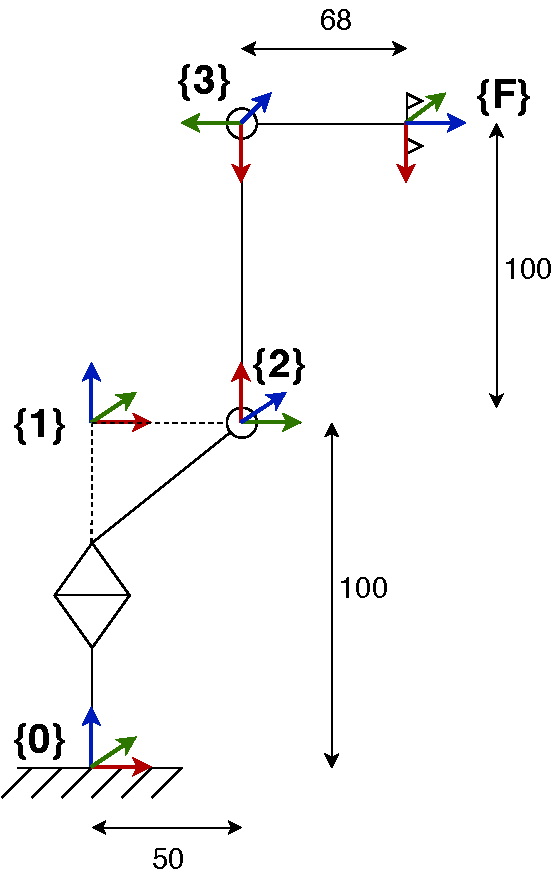
\includegraphics[width=0.35\columnwidth]{images/robot_axis_coord.pdf}
	\caption{axis coordinate systems for computing the inverse kinematic}
	\label{fig:robot-axis-coord}
\end{figure}



%-------------------------------------------------------------------------------
\section{Tool Calibration}
The tool calibration includes three steps: Estimating the camera projection matrix as well as the transformation from the main camera (left in robot sight direction) to the TCP and the transformation of the laser pointer towards the TCP. 

\subsection{Hand-Eye Transformation Matrix}
The hand-eye calibration is measured from the real robot. It is assumed, that the rotation between the camera coordinate system and the tool is small. We only have to rotate the coordinate system and take the translation vector into account. Another method would be that of Park and Martin \cite{ParkHandEye} which is also provided in OpenCV. 

\begin{figure}[h]
	\centering
	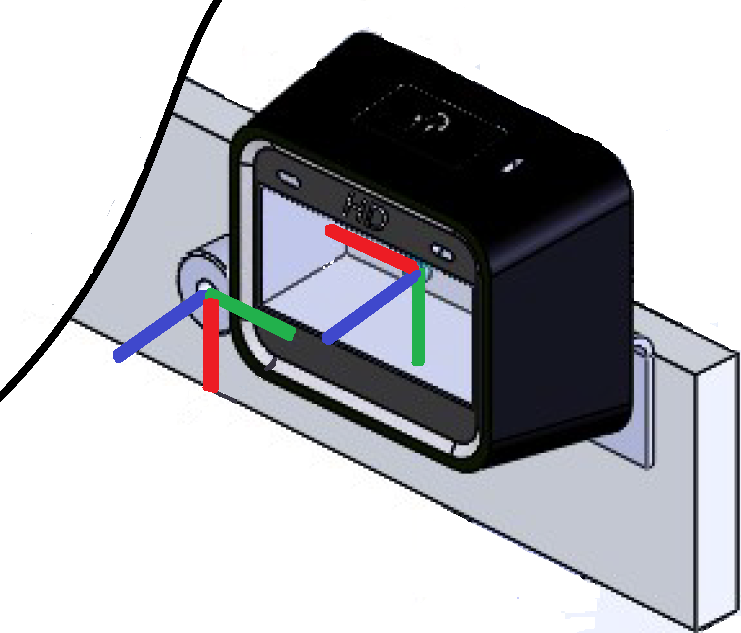
\includegraphics[width=0.3\columnwidth]{images/hand_eye_coord_2.png}
	\caption{axis coordinate systems for computing the backwards kinematic}
	\label{fig:hand_eye_coord}
\end{figure}

\subsection{Laser Calibration}
Since the laser is designed to lay directly in line with the Z-coordinate of the tool frame, there is no calibration needed. This demands a fine level of accuracy for the manufacturing process. 

\subsection{Stereo Camera Projection Matrix}

The camera projection matrix is estimated from multiple images of the same chessboard calibration plate \cite[p. 178-182]{Ziss2008}. At first, the intrinsic parameters of both cameras are estimated separately using the OpenCV function \textit{calibrateCamera}. With this information the function \textit{stereoCalibrate} can be used to estimate the translation and rotation between the two cameras. With these matrices and the function \textit{triangulate} a 2D point correspondence can be associated with one 3D point. The camera calibration app is implemented in Python using these OpenCV functions \cite{2014opencv}. 



%-------------------------------------------------------------------------
\section{Object Detection}
Two methods for detecting the laser dot are tested.  \\
\textbf{Option 1:} use a HSV-threshold and only look for pixels with that specific value. This method is unstable against different illumination scenarios. \\
\textbf{Option 2:} use template matching with user-defined template. The main idea is to calculate a normalized difference between every pixel in the image and a template \cite[p. 1061-1062]{Gonz2018}. This function is called \textit{matchTemplate} and is also provided by OpenCV. The method \textit{CV\textunderscore TM\textunderscore CCOEFF\textunderscore NORMED} was found to work most reliable for multiple different lighting scenarios. This method uses the equation \ref{eq:template_matching} below, where $T$ stands for the template and $I$ is the image. 


\begin{equation}
R(x,y) = \frac{\sum_{x',y'} (T'(x',y') \cdot I'(x + x', y + y'))}{\sqrt{\sum_{x',y'} T'(x',y')^{2} \cdot \sum_{x',y'} I'(x + x', y + y')^{2}}}
\label{eq:template_matching}
\end{equation}




%-------------------------------------------------------------------------
\section{Result and Conclusion}
We can show that the described system works as specified. We find, that template matching is better suited to detect small objects in a constantly changing image rather than searching the images for a specific colour.  
Further steps could include to verify the assumption about the orientation of the laser tool as well as refining the hand-eye calibration. 


%-------------------------------------------------------------------------{\small
{\small
\bibliographystyle{ieee}
\bibliography{acvrw}
}

\end{document}
